\documentclass[10pt]{article}

\usepackage{amsmath}
\usepackage{amssymb}
\usepackage{graphicx}
\usepackage{subcaption}

\begin{document}
\title{Project 1 Report}
\author{Chau Tran | Adrian Duric | Preben Castberg\\\footnotesize\texttt{cttran@uio.no} | \texttt{adriandu@uio.no} | \texttt{prebennc@uio.no}}
\date{04/09/2025}
\maketitle

\begin{abstract}
  This is an example. Use this template as a starting point for writing your report for project 1. The abstract is usually between 100-400 words, and should summarize the contents of your report. In short, state the problem and the methods you have used, and give your results and conclusion.
\end{abstract}

\section{Introduction}
Use the introduction to describe the problem, the methods you will apply to investigate or solve it, any hypotheses you have, and outline your findings.
How you organize the text is up to you, but keep in mind that you are in a sense telling the story of how your project went (without the gritty details). You want to capture the interest of the reader and then keep them interested enough to read your whole paper!
Why is the problem relevant? How are the results useful? What are the implications of your results?
Imagine that you are trying to ``sell'' your ``product'' (i.e. your project and results).
Feel free to use the problem description in the \texttt{project-1} document as a starting point.

\section{Related Work}
In this section, you contextualize your project by referring to other research that inspired, is similar to, or is otherwise related to your own.
We don't expect you to give a super detailed overview of all research about adaptation methods and ViTs that exists out there, but you can for example try to find some research on the performance of LoRA in different settings.
Put your references in the \texttt{report.bib} file. There should be an example there already \cite{Test}.

\section{Low-Rank Adaptation}
\label{sec:lora}

Low-Rank Adaptation (LoRA) is a method that, given some pretrained weights in a neural network, indirectly continues to train the weights by freezing them, and then updating a new set of auxiliary weights which represent the change of the original weights \cite{hu2021loralowrankadaptationlarge}. Assume we have a pretrained layer of model weights $W_0 \in \mathbb{R}^{d \times k}$. LoRA indirectly updates this layer as $W_0 + \Delta W$, where $\Delta W = BA$ such that $B \in \mathbb{R}^{d \times r}$, $A \in \mathbb{R}^{r \times k}$ and $r \ll min(d, k)$ is the rank. When training the model with LoRA, $W_0$ is frozen so that only the weights in $A$ and $B$ are updated. For some input vector $x$ which would otherwise be projected as $h = W_0x$, the LoRA-based projection instead becomes:

\begin{equation}
    h = W_0x + \Delta Wx = W_0x + BAx
\end{equation}

Since both terms $W_0x$ and $BAx$ produce output vectors of the same dimensions, these vectors are summed elementwise, producing $h$.

Upon beginning training with LoRA, $A$ is initialized with randomly sampled parameters from the Gaussian distribution, while $B$ is zero-initialized, meaning $BA$ is also zero when training begins. Notice that $W_0$ contains $d \cdot k$ parameters, while $BA$ contains $d \cdot r + r \cdot k = r(d + k)$ parameters. Since $r \ll min(d, k)$, updating $\Delta W = BA$ becomes computationally cheaper to update than $W_0$, while also requiring less memory than $W_0$ to store the parameters; it can even reduce total memory usage, since no gradients need to be kept in memory for $W_0$. This makes it inexpensive to store a finetuned model with the added LoRA decomposition for deployment in production tasks.

\section{Experiments and Results}
In this section you outline the experiments you have ran, and present the results.
In general, we encourage the use of tables, graphs, and figures.

\subsection{Finetuning ViT on ImageWoof}
\label{subsec:finetuning_vit_imagewoof}

To have a baseline performance level to which we can compare LoRA, we first finetuned a pretrained ViT \cite{dosovitskiy2021imageworth16x16words} model on the ImageWoof dataset, a subset of the ImageNet \cite{deng2009imagenet} dataset consisting of images from 10 different dog breeds. Relative to ImageNet, which contains a wide range of different image subjects, ImageWoof is more finegrained in the sense that the visual differences between different dog breeds tend to be more subtle than those between, say, a dog and a car. Differentiating between visual features that separate different dog breeds, or other similarly-looking sets of classes, is therefore typically considered a harder visual classification task than doing classification on broader-ranging sets of classes like in ImageNet.

We used the \verb|vit_tiny_patch16_224| implementation of ViT provided by the \verb|timm| \cite{rw2019timm} model library, which is pretrained on ImageNet-21k and finetuned on ImageNet2012. We replaced the classification head with one for each of the 10 ImageWoof classes. We resized each image to $224 \times 224$ pixels, and applied channelwise normalization. During training, we also randomly cropped the input images. We used a batch size of 64, and optimized using stochastic gradient descent with a learning rate of 0.001 and the cross-entropy loss function. We measured and present top-1 validation accuracy after training the model for 5 epochs on ImageWoof.

\subsubsection{Results}

We present the total training time for the standard ViT model with 5 epochs of finetuning on ImageWoof, and accuracy on the validation set. We also present curves showing the progression of training accuracy and loss.

\begin{table}[ht]
    \centering
    \begin{tabular}{c|c}
        Accuracy (\%) &  92.2 \\
        Training Time (minutes) & 18.66
    \end{tabular}
    \caption{Accuracy and training time for ViT on the ImageWoof validation set after finetuning.}
    \label{tab:placeholder}
\end{table}

\begin{figure}[ht]
    \centering
    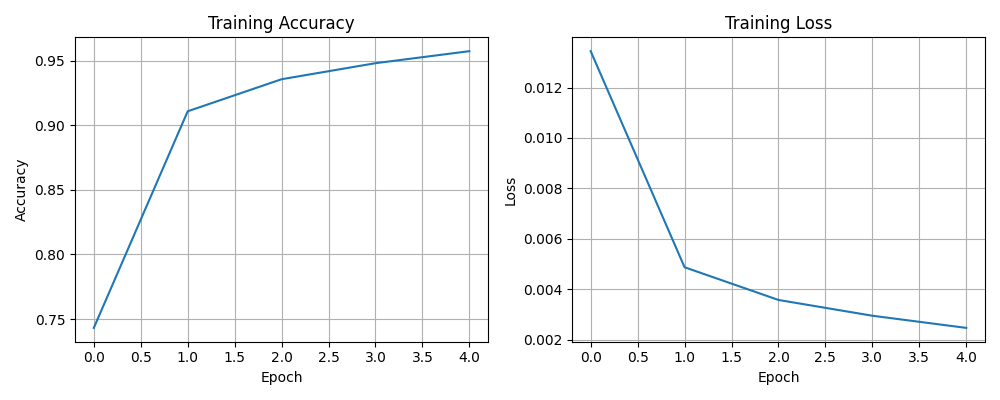
\includegraphics[width=1\linewidth]{images/training_loss_curve_vanilla.png}
    \caption{Training loss and accuracy with standard ViT on ImageWoof over 5 epochs.}
    \label{fig:placeholder}
\end{figure}

From the graphs, we observe normal behavior from the model during training. These results are compared to ViT + LoRA results in Section \ref{res_lora}.

\subsection{Finetuning ViT + LoRA on ImageWoof}

Having collected a baseline performance measurement from the standard ViT model, we then measured performance under the same circumstances when using LoRA to finetune the ViT model instead.

We implemented LoRA by freezing all layers except the classification head of the ViT. Then for the linear layers of each attention block, we initialized auxiliary linear tensors $A$ and $B$ as described in Section \ref{sec:lora}, and let $A$ and $B$ be unfreezed so their parameters can be updated. We initialized them with rank $r = 4$, one of the rank values used in the original LoRA paper \cite{hu2021loralowrankadaptationlarge}. We otherwise followed the exact same experimental configuration as detailed in Section \ref{subsec:finetuning_vit_imagewoof}.

\subsubsection{Results}
\label{res_lora}

We present the total training time for the ViT + LoRA model with 5 epochs of finetuning on ImageWoof, and accuracy on the validation set. We also present curves showing the progression of training accuracy and loss.

\begin{table}[ht]
    \centering
    \begin{tabular}{c|c}
        Accuracy (\%) &  83.0 \\
        Training Time (minutes) & 18.69
    \end{tabular}
    \caption{Accuracy and training time for ViT + LoRA on the ImageWoof validation set after finetuning.}
    \label{tab:placeholder}
\end{table}

\begin{figure}[ht]
    \centering
    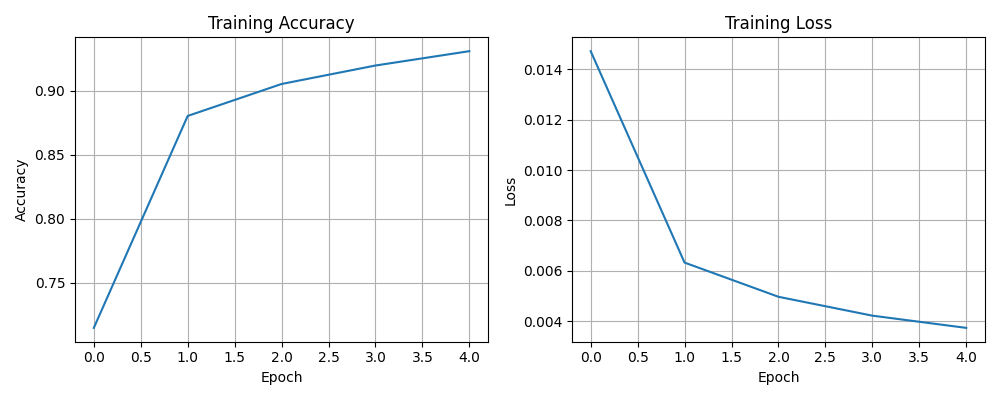
\includegraphics[width=1\linewidth]{images/training_loss_curve_LoRA.png}
    \caption{Training loss and accuracy with ViT + LoRA on ImageWoof over 5 epochs.}
    \label{fig:placeholder}
\end{figure}

We observe that the ViT + LoRA accuracy is significantly lower on the ImageWoof validation set than when using the standard ViT. This is surprising, given that the graphs of training accuracy and loss show similar values across epochs with only a minor dropoff of a couple of percentage points. In terms of training time, the two models were almost exactly equal.

\subsection{Visualizing Attention Maps}
Visualize the final attention maps of the ViT. How does the attention changes from the original ViT to the ViT+LoRA model?

The attention mechanism in Vision Transformers (ViTs) allows the model to focus on different parts of an image when making predictions. To understand what the model ``looks at,'' we visualize these attention maps. Using functions provided in the \textit{w2\_ViT\_DINO\_DEMO} notebook, the models are slightly modified to capture the attention weights from the last attention layer, which is typically the most informative for classification tasks.

The \texttt{attention\_forward\_wrapper} function overrides the forward pass of an attention layer. While keeping the core computation logic intact, it stores the attention probabilities in \texttt{attn\_map}, allowing us to access the attention maps later without interfering with the model's normal predictions. The last attention block of each model is patched to use this wrapper, so every forward pass automatically saves the attention map for the CLS token.

To extract meaningful visualizations, the attention of the CLS token over all image patches is selected and averaged across all attention heads. This patch-level attention is reshaped into a square grid corresponding to the patch layout, upsampled to match the original image size, and normalized to a [0, 1] range. The resulting heatmap can then be visualized using two helper functions. The \texttt{show\_img\_overlay} function overlays the attention map on the original image with adjustable transparency, while \texttt{show\_img\_size\_by\_size} creates a side-by-side comparison showing the original image, the attention map alone, and the overlay. These visualizations provide insights into which parts of the image the model focuses on, giving a better understanding of the inner workings of transformer models.

An example of how the attention maps look in both Vanilla ViT and ViT with LoRA is shown in Figure~\ref{fig:attentionmaps}. It compares the attention maps of a Vanilla ViT and a ViT enhanced with LoRA. In the Vanilla ViT, the attention is highly concentrated on a single region of the image, focusing strongly on the most discriminative feature of the object. By contrast, the ViT with LoRA produces a more distributed attention pattern, highlighting not only the main region but also capturing additional relevant details of the object. This suggests that LoRA encourages the model to become slightly more context-aware, balancing between strong focus and richer feature coverage.

\begin{figure}[htbp]
    \centering
    % Top subplot
    \begin{subfigure}[b]{0.9\textwidth}
        \centering
        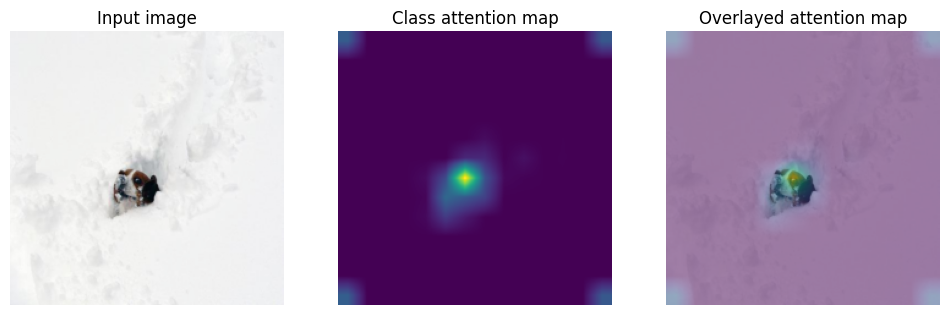
\includegraphics[width=\textwidth]{images/vit_attention.png} % replace with your image
        \caption{Vanilla ViT Attention Map Sample}
        \label{fig:vit_attentionmap}
    \end{subfigure}

    \vspace{0.5cm} % optional space between subplots

    % Bottom subplot
    \begin{subfigure}[b]{0.9\textwidth}
        \centering
        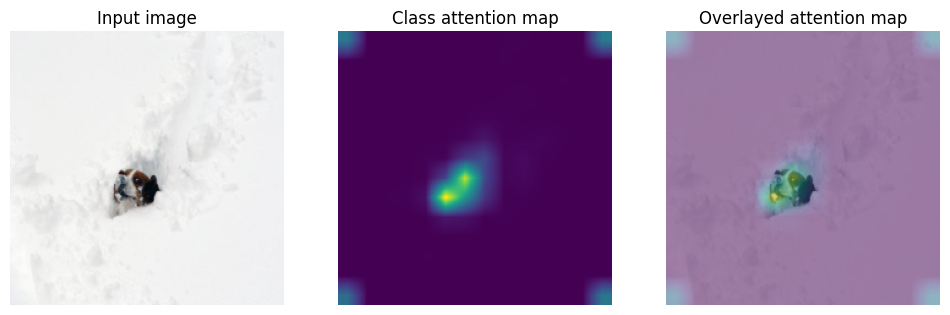
\includegraphics[width=\textwidth]{images/lora_attention.png} % replace with your image
        \caption{ViT with LoRA Attention Map Sample}
        \label{fig:lora_attentionmap}
    \end{subfigure}

    \caption{An example of attention maps created from the vanilla ViT and Vit with LoRA.}
    \label{fig:attentionmaps}
\end{figure}

\section{Discussion}
Here you discuss the results of your experiments. Did it match your initial hypotheses? Why/why not? What are the implications of the results?

\section{Conclusion}
State your conclusion to tie up the report. This is else where you can mention the direction of future work based on the results of this one.

From the first two experiments, we observed a significant dropoff in accuracy with ViT + LoRA compared to standard ViT, while the training times were almost equal.

\section{Group Contributions}

For the programming, Adrian wrote the code for the LoRA wrapper, freezing and unfreezing relevant parts of the models and the training and testing of the models. Preben wrote the code for conducting the first two experiments and obtaining result metrics that were presented in this report. Chau wrote the code for visualizing the attention maps with and without LoRA, the third experiment.

For the report, Preben wrote the abstract, introduction and related work parts. Adrian wrote the methods part, as well as the experiment and results and conclusion parts regarding the first two experiments. Chau wrote the equivalent parts for the third experiment, as well as the discussion part.

\bibliographystyle{IEEEtran}
\bibliography{report}

\end{document}